plate \graphicspath{{chapters/6.Chapter_4/figures/}}

\begin{savequote}[75mm]
In biology, nothing is clear, everything is too complicated, everything is a mess, 
and just when you think you understand something, you peel off a layer and find 
deeper complications beneath. Nature is anything but simple.
	\qauthor{- Richard Preston: The Hot Zone}
\end{savequote}

\chapter{RNAi in \textit{P. bursaria}}

\section{Introduction}

\subsection{RNAi}

Post-transcriptional gene silencing (PTGS) is a highly useful experimental technique
in reverse genetic analysis of a given gene.  
The most widely used PTGS method is that of RNA-mediated inteference (RNAi)
of gene expression. 
RNAi \citep{Fire1998} is a powerful experimental technique which is widely used 
in the study of model eukaryotic organisms \citep{Morf2013,Batista2011,Matthew2004,Ketting2011,Chang2012}.

RNAi covers a set of evolutionarily conserved mechanisms across the eukaryotes 
with numerous mechanisms in which the expression of particular transcripts
is regulated via several classes of transcribed small non-coding RNA (ncRNA)
such as short-intefering (siRNA), micro (miRNA) and Piwi-interacting (piRNAs) \citep{Carthew2009}.

These systems likely originated as a form of defence against
viruses and transposons \citep{Waterhouse2001,Buchon2006}
and were present in some form in the last universal eukaryotic
ancestor (LECA) \citep{Cerutti2006,Shabalina2008}.  Many eukaryotes
utilise these small RNA-mediated gene silencing pathways
in the regulation of their own cell expression patterns \citep{Wu2008}.
Despite its ancestral nature there has been considerable diversification
of both this process, its function and mechanism \citep{Ketting2011}.
Indeed, even with the same organism, different points of the life cycle
may use different RNAi systems \citep{Flemr2013}.


Generally RNAi pathways involve the generation of 21-28nt short RNAs
from some form of RNA precursor such as dsRNA (or ssRNA)
via the function of the RNAase III Dicer \citep{Bernstein2001} or related proteins.
These short RNAs are then bound by Argonaute proteins which act alone or as part
of a complex to silence the expression of sequences homologous to the siRNA \citep{Ketting2011}.
This silencing isn't just limited to the post-transcriptional endonucleocytic degradation of 
mRNA transcripts but can also involve transcriptional inhibiton and
DNA elimination \citep{Marker2014}.
The one unifying element of all discovered RNAi pathways is that
of the central role argonaute (AGO) proteins play \citep{Ketting2011}.
They are formed of two subclasses: the Ago and Piwi subfamilies \citep{Peters2007}
with a range of functions and complex-forming behaviours
\citep{Ender2010}.
The magnitude of the silencing response is occasionally amplified by the generation
of more copies of the trigger dsRNA by RNA-dependent RNA polyermases (RdRPs) \citep{Arp2007}.
On the other hand RdRPs can also sometimes directly generate the siRNAs \citep{Aoki2007,Ketting2011}.
Interestingly, the last universal eukaryotic ancestor (LECA) likely contained 
at least one Ago and Piwi family Argonaute protein, a Dicer and an RdRP \citep{Cerutti2006}.

The two main systems are the siRNA and miRNA based systems.  They are differentiated
by miRNAs being encoded by dedicated genes and displaying partial
complementarity to their targets whereas siRNAs are generated from exogenous
dsRNAs (i.e. environmental dsRNA from viral infection or phagocytosed bacteria \citep{Whangbo2008})
or transgenes and involve full or near full complementarity \citep{Shabalina2008}
However, there are also piRNA systems involved in germline based transposon silencing \citep{Iwasaki2015}.
An important ciliate specific system is that of scan RNAs (scnRNAs) which 
are involved in the elimination of internal eliminated sequences (IESs) during
macronuclear (MAC) regeneration \citep{Mochizuki2004,Chalker2013}.


Experimentally, the existence and function of these systems
permits a researcher to introduce dsRNA homologous to an RNA transcript of interest
and trigger targeted cell-wide RNAi of that transcript.
Unforunately, there also several problems with RNAi as a general method.
Many organisms lack active RNAi systems, although such systems can occasionally
be induced \citep{Alibu2005}.
On top of this, RNAi requires exact sequences to design precursors.
In order to minimise off-target effects, in which a provided sRNA precursor induces RNAi
in more than just the target transcript, a complete genome and/or transcriptome
is useful in the design stage as off-target hits can be checked. 
Off-target effects  can lead to cryptic
phenotypic outcomes that are then falsely attributed to the initial target.
Another problem is that RNAi does not necessarily induce total silencing
of a given transcript and low-levels of transcription may still occur.
This, conceivably, can be sufficient to maintain the non-knock down phenotype.

\subsection{RNAi in \textit{Paramecium}}

In addition to the scnRNA system mentioned above siRNA
based pathways have been discovered in the two principal
ciliate model organisms: \textit{Tetrahymena thermophila} \citep{Collins2006,Yao2005}
and \textit{Paramecium tetaurelia} \citep{Galvani2001,Galvani2002}. 
There are 2 established methods for inducing RNAi in \textit{Paramecium tetaurelia}:
microinject and transformation of the MAC with high-copy transgenes lacking 3' untranslated
region (UTR) \citep{Galvani2001} and the introduction of dsRNA by either
microinjection or feeding using transformed dsRNA expressing bacteria 
\citep{Galvani2002}.

In the transgene pathway, the 3' truncation to the production of aberrant
sense and antisense transcripts \citep{Galvani2001,Marker2010,Beisson2010b}.
Based on the identified required components (see \cref{tab:marker_components}), 
aberrant transcripts
are processed by a Dicer protein (Dcr1) \citep{Lepere2009} and
an putative RdRP complex formed of an RdRP (Rdr2) and a nucleotidyl
transferase (Cid2) \citep{Marker2014} into 23nt siRNA \citep{Lepere2009}. 
A putatively non-catytic 
RdRP (Rdr3) also plays an undefined role in the generation
of primary (\(1^{\circ}\)) siRNAs from transgene pre-cursors \citep{Marker2010,Marker2014}.
Finally, two Argonaute Piwi proteins (Ptiwi13 and Ptiwi14) \citep{Bouhouche2011} 
are involved in targeting post-transcriptional silencing via mRNA
cleavage \citep{Bouhouche2011,Marker2014}.


Alternatively, the exogenous dsRNA pathway can be induced by either microinjection directly
into the MAC (for a transient 48 hour long silencing) or by continue feeding
with a bacterially experimentally modified to generate dsRNA.
Typically, this involves an \textit{E. coli} 
with an IPTG-inducible T7 polymerase and 
deficiency for RNAse III containing a plasmid with a T7 promoter and sequence
homologous to the target transcript
\citep{Fire1998,Timmons2001,Galvani2002}.
Interestingly, there is some evidence that this pathway also is activated at low
levels by ssRNA from normal food bacteria \citep{Carradec2015}.

\begin{table}
    \centering
    \begin{tabular}{|c|c|c|}
        \hline
        \textbf{Pathway} & \textbf{Component} & \textbf{Function} \\
        \hline
        transgene-induced siRNA & Rdr3 & RdRP \\
                                & Ptiwi14 & Piwi \\
        both pathways           & Rdr2 & RdRP \\
                                & Dcr1 & Dicer \\
                                & Ptiwi13 & Piwi \\
                                & Cid2 & Nucleotidyl transferase \\
        exogenous dsRNA-induced siRNA & Rdr1 & RdRP \\
                                      & Cid1 & Nucleotidyl transferase \\
                                      & Ptiwi12 & Piwi \\
                                      & Ptiwi15 & Piwi \\
                                      & Pds1 & Import of dsRNA? \\
        \hline
    \end{tabular}
    \caption[Summary of RNAi pathway components in \textit{P. tetaurelia}]{Summary
        of the components identified as necessary to the function of both
        primary siRNA RNAi pathways in \textit{P. tetaurelia} as identified
        by forward genetic screens in \citep{Marker2014}}
    \label{tab:marker_components}
\end{table}


Again, based on the components that have been identified as necessary
for this exogenous dsRNA pathway to function (see \cref{tab:marker_components}).  
RNA precursors are processed
by Dcr1 \citep{Lepere2009}, and then two hypothetical RdRC (Cid1-Rdr1, Cid2-Rdr2)
\citep{Marker2010,Marker2014} are involved in the generation of \(1^{\circ}\) 
siRNA.  
The second RdRC (or specifically Rdr2) is also involved in the generation
of low levels of secondary (\(2^{\circ}\)) siRNA which spread along the full length of
target mRNA (i.e. 3'-to-5' and 5'-to-3' transitivity) in primarily
antisense form \citep{Carradec2015}.  These \(2^{\circ}\) siRNAs don't
appear to play a significant role in silencing themselves (contrary to similar
systems in \textit{C. elegans} where they form the principal targetter of silencing 
\citep{Sijen2007,Pak2007}) \citep{Carradec2015}.
3 Piwis play a role in targeting silencing.  Ptiwi13 hypothetically
loads the \(1^{\circ}\) siRNA and targets cleavage of cytoplasmic mRNA \citep{Bouhouche2011},
while Ptiwi12 and Ptiwi15, based on their homology to nuclear Piwi proteins,
\citep{Marker2014,Carradec2015,Bouhouche2011} may be involved
in \(2^{\circ}\) siRNA communication with the MAC \citep{Carradec2015}.
One final protein necessary for the function of feeding based dsRNA-induced
RNAi is an uncharacterised novel \textit{P. tetaurelia} complex protein (Pds1) \citep{Marker2014}.
It has been hypothesised that this may play a role in the export of RNA from 
the food vacuole \citep{Carradec2015}.


Many of these components are a product of the 3 whole genome duplication
events in the evolution of the \textit{Paramecium} clade \citep{McGrath2014}.
As \textit{P. bursaria} shares only the first \textit{Paramecium} clade whole
genome duplication event with \textit{P. tetaurelia} it is expected
it should contain the RNAi components identified as belonging to WGD1 (or have 
secondarily lost them) \citep{McGrath2014}.
This is believed to include a single RdRP gene, 6 Piwi genes, and 2 Dicer genes \citep{Marker2014}.

%siRNAs are made endogenously from an intergenic lopcus of unknown functions \citep{Marker2010,Marker2014}
%exogenous ssRNAmay protect against horizontal transfer of ss retroelements \citep{Carradec2015}

%Although the clustered regularly interspaced short palindromic repeat (CRISPR)/Cas
%system can be used to simplify gene editing or deactivation (CRISPRi).
%This system is not available in \textit{Paramecium}.

If it is possible to experimentally induce RNAi in \textit{P. bursaria} CCAP 1660/12
specific hypotheses as to the necessity of hypothetically important
endosymbiotic components can be tested. For example, what is the effect
on the endosymbiosis of the inhibition of certain host-derived transporters.

Similarly, what components of core \textit{P. tetaurelia} RNAi pathways
can be identified 
in the \textit{P. bursaria} - \textit{M. reisseri}/\textit{C. variabilis} transcriptomes?
Are they being expressed during endosymbiosis?  Can they be found in the incomplete
CCAP 1660/12 MDA genome contigs?

\subsection{``Cross-talk''}

Evidence has emerged of the role of RNAi in numerous host-pathogen 
\citep{Nowara2010,LaMonte2012,Weiberg2013,Buck2014}
and host-symbiont \citep{Helber2011,Koch2013} relationships.
This has led some authors to suggest that sRNA and RNAi mechanism form an import
mechanism of cross-talk between diverse organisms and even across
domains \citep{Liang2013,Knip2014,Weiberg2015}.

The evidence of natural food bacteria ssRNA induced RNAi in \textit{P. tetaurelia}
\citep{Carradec2015} implicates a potential important role for cross-talk
in \textit{P. bursaria} regulation. Compounding this with the fact
that \textit{P. bursaria} in addition to being a serial phagotroph
it also contains numerous bacterial and green algal endosymbionts.
Therefore, merely from the perspective of ``attack surface'' there is a plausible
role for cross-talk occurring in \textit{P. bursaria}.   Therefore, 
it may be informative to investigate the quantity and targets of
potential cross-talk between host and endosymbiont in terms of 
``collisions''  i.e. matching 23nt RNA strings between host and endosymbiont
transcripts bins.   Contextualising these these values 
across the diversity of the tree of life is important.
``Collision'' levels have implications for the regulation and expression of exogenous dsRNA
RNAi pathways by the host. 
%While a \textit{Paramecium} virus is yet to be discovered there
%are evidence of the association of \textit{Paramecium bursaria-Chlorella} Viruses
%with the system therefore, it is not inconceivable that these may play some role.  


\section{Aims}

The goal of this chapter is to investigate both the practical and
theoretical utility of RNAi systems in \textit{P. bursaria}. 
Specifically:
\begin{itemize}
    \item Is \textit{P. bursaria} capable of microinjection or feeding based
        exogenous dsRNA siRNAi?
    \item What components, previously identified as necessary, for these pathways
        are present and expressed in \textit{P. bursaria}? 
    \item Is there any possible explanation for the deactivation of one or other
        of these systems? 
\end{itemize}


\section{Methods}

\subsection{RNAi constructs}

All RNAi methods were based on previously published protocols specifically,
\citep{Galvani2001,Galvani2002,Beisson2010}.

6 different constructs were created featuring a genes whose knock-down
has previously established phenotypes in \textit{P. tetaurelia} (see \cref{tab:rnai_vecs}).
All inserts were designed in the same manner, \textit{P. tetaurelia} sequences
were taken from the \textit{P. tetaurelia} genome. 
These were then BLASTN against the entire unbinned \textit{P. bursaria}-\textit{M. reissieri}
CCAP 1660/12 transcriptome and designed based on the \textit{P. bursaria} sequence.
Each insert was cloned into an L4440 vector featuring two convergent T7 promoters
featuring an ampicillin resistance marker. 


\begin{table}
    \begin{tabular}{|c|c|c|c|c|}
        \hline
    \textbf{Gene} & \textbf{Function} & \textbf{RNAi phenotype in}      & Vector Design & Reference \\
                  &                   & \textbf{\textit{P. tetaurelia}} &               &           \\
        \hline
        \textit{epi2} & Epiplasmin & ``Monstrous'' cells  & 500bp via \textit{Pst}I and \textit{Hind}III & \citep{Damaj2009} \\
        NSF & Membrane fusion factor & Lethal & 500bp via \textit{Pst}I and \textit{Hind}III & \citep{Galvani2002} \\
        pTMB.422c & Binding protein & Lethal & 500bp via \textit{Pst}I and \textit{Hind}III & \citep{Nowack2011} \\
        \textit{bug22} & Basal body/ciliary protein & Slow swimming and death & 313bp via \textit{Xba}I and \textit{Hind}III & \citep{Laligne2010} \\
        BBS7 & Ciliary ion transport & Fewer, shorter ciliar & 486bp via \textit{Xho}I and \textit{Hind}III & \citep{Valentine2012} \\
        PGM & PGM endonuclease & Post-autogamous cells unable to resume normal growth & 500bp via \textit{Pst}I and \textit{Hind}III & \citep{Baudry2009} \\
        \hline
    \end{tabular}
    \caption{Details of RNAi vectors used.  All constructs were cloned into a L4440 vector and used an Ampicillin resistance market}
    \label{tab:rnai_vecs}
\end{table}

\subsubsection{RNAi feeding}

For feeding experiments the vectors were transformed into \textit{E. coli} HT115-DE3.
This strain is deficient for RNAse III and features an IPTG inducible T7 polymerase
under the control of a Plac promoter. Method used was derived from ParameciumDB, 
published \citep{Beisson2010}.

Bacterial precultures were started using a single colony picked from an LB
plate containing \(50\mu gml^{-1}\) ampicillin and \(12.5\mu g ml^{-1}\) tetracyline.
This picked colony was grown overnight in LB medium with the same antibiotics.
The overnight cultures was then diluted 50 fold and grown with shaking
at \(37\celsius\) up to an \(OD_{600}\) of 0.4 to 0.6. IPTG
was then added at a concentration of 0.4mM and shaken for 3 hours
at \(37\celsius\).  30ml of this culture was centrifuged for 2 minutes (3100 x g),
then the supernatant removed and the pllete washed twice in \textit{Paramecium}
growth medium. The pellet was resuspended in \textit{Paramecium} medium with 0.4mM IPTG,
\(100\mu g ml^{-1}\) ampicillin and adjusted to a final \(OD_{600}\) of 0.1.
\(1 \mu l\) of beta-sitosterol (at \(4mg ml^{-1}\) in ethanol) was added
to each 5ml of medium.

For the actual feeding, \(10ml\) \textit{P. bursaria} CCAP 1660/12 culture
was centrifuged at 800x g for 10 minutes and re-suspended in \(1ml\) of supernatant.
\(9ml\) of the induced bacterised media was then added.  The sample was
then incubated in a tissue culture flask at \(27\celsius\).
Feeding was repeated for each day of analysis. 

\subsubsection{RNAi microinjection}

Microinjection used the same protocol as described in \citep{Beisson2010b} 
but only tested the PGM construct.
Briefly, the circular plasmid is linearised using a unique restriction site,
and purified using phenol:ethanol extraction and a purification column.
It is then dissolved in \(H_{2}O\) at a mininmum concentration of 
\(5mg ml^{-1}\).
Cells were washed twice by picking with a micropippete in Dryl-BSA wells before
being placed into inidival droplets on a glass coverslip and covered in paraffin oil.
The coverslip was then placed onto a microscopy stage and a microinjector 
used under 10X mangification to inject linearised construct directly into the
macronucleus.

\subsection{Analysis of RNAi pathway}

\subsubsection{Survey for RNAi components in \textit{P. bursaria}}

Using the canonical seed sequences identified in \textit{P. tetaurelia}
by \citep{Marker2014} (see \cref{tab:rnai_seeds}) the entire assembled 
\textit{P. bursaria}-\textit{M. reisseri} CCAP 1660/12 transcriptome,
\textit{P. bursaria}-\textit{C. variabilis} YADG1N transcriptome
and the assembled \textit{P. bursaria}-\textit{M. reisseri} CCAP 1660/12
genomic contigs over 500bp were searched using tBLASTn
with a minimum expectation threshold of \(1e^{-5}\).

\begin{table}
    \centering
    \begin{tabular}{|c|c|c|c|}
        \hline
        \textbf{Gene} & \textbf{\textit{P. tetaurelia} Accession} & \textbf{Length} \\
        \hline
        Rdr1 & PTETG8500012001 & 4319 \\ 
        Rdr2 & GSPATG00036857001 & 4162 \\
        Rdr3 & GSPATG00006401001 & 3292 \\
        Cid1 & PTETG9100013001 & 1051 \\
        Cid2 & PTETG13400003001 & 1083 \\
        Pds1 & PTETG600032001 & 2084 \\
        Dcr1 & GSPATG00021751001 & 5394 \\
        Ptiwi12 & GSPATG00001709001 & 2315 \\
        Ptiwi13 & PTETG4800007001 & 2483 \\
        Ptiwi14 & PTETG16300003001 & 2428 \\
        Ptiwi15 & GSPATG00005370001 & 2315 \\
        \hline
    \end{tabular}
    \caption[RNAi pathway components from Marker]{\citep{Marker2014}}
    \label{tab:rnai_seeds}
\end{table}

Additionally, the other sequenced \textit{Paramecium} genomes 
were searched using BLASTP via ParamediumDB \citep{Arnaiz2007,Arnaiz2011a}.
Specifically, \textit{P. caudatum} \citep{McGrath2014}, 
\textit{P. biaurelia}, \textit{P. primaurelia}, \textit{P. sexaurelia}
and \textit{P. multimicronucleatum}. Finally,  \textit{T. thermophila} 
predicted proteins were also searched \citep{Eisen2006}.


\subsubsection{Phylogenetic analysis of RNAi pathway}

Hits for each seed in the databases searched were then converted
to peptides based on the reading frame of the top hit. The ORF containing the
hit was extracted for genomic hits. 

Peptide sequences were then aligned using MAFFT \citep{Katoh2002} and manually
masked using Seaview \citep{Gouy2010}.
An LG+\(\Gamma_8\) sequence evolution model was then selected on the basis
of AICc in Prottest3 \citep{Darriba2011a}.
Phylogenies were then generated using RAxML with 1000 non-rapid bootstraps and MrBayes 
with 2 runs of 4 MCMCMC chains run for 2,000,000 generations or until convergence.
Aberrant sequences such as long branches or were then removed, the sequences
re-aligned and phylogenies regenerated.


\subsection{Cross-Talk Analysis - ``eDicer''}

In order to investigate the prevalence of ``cross-talk'' between 
host and endosymbiont a tool to analyses short sequence collisions between two sets
of transcripts was created.  ``eDicer'' is built upon Jellyfish \citep{Marcais2011}
and the K-mer Analysis Toolkit (KAT) \citep{ClavijoKAT}.  It allows
the comparison (and normalisation) of the number of Dicer fragment collisions
between a set of transcripts and a list of transcript sets from organisms
of choice for a given dicer fragment size.  
For each query transcript set in this list the following
values are calculated and tabulated:
\begin{itemize}
    \item Number of K-mers in the query, in other words the length of the query
        in K-mers (\(\frac{\sum^s_{n=1} len(x_{n}}{len(w)}\)
        for a set containing \(s\) transcripts and a K-mer size of \(w\)).
    \item Number of unique K-mers in the query, the non-redundant length of 
        the query.
    \item Number of shared  K-mers (``collisions'') between query and subject bin.
    \item Number of unique shared K-mers betwee query and subject bin.
    \item Shared K-mers normalised by subject length in K-mers.
    \item Shared K-mers normalised by the subject length in unique K-mers.
    \item Shared unique K-mers normalised by subject length in K-mers.
    \item Shared unique K-mers normalised by the subject length in unique K-mers.
\end{itemize}

In this case, I examined all 23-mer collisions between endosymbiont 
and host transcriptomes. In order to contextualise these
values I also compared the endosymbiont transcripts with 
sets of transcripts (or CDS) from taxa representative of the 
sequenced diversity of each of the
following groups: bacteria, archaea, eukaryotes, green algae, ciliates,
and host transcripts from \textit{P. bursaria} SW1 and \textit{P. bursaria} Yad1g.

Specifically, 3 ciliate sets were used \textit{Paramecium tetaurelia}, 
\textit{Tetrahymena thermophila} and \textit{Oxytricha trifallax} along with
5 green algae \textit{Chlamydomonas reinhardtii}, \textit{Coccomyxa subellipsoidea}
C-169, \textit{Chlorella variabilis} NC64A, \textit{Micromonas pusilla} RCC299, and
\textit{Ostreococcus lucimarinus}.
Additionally, 58 eukaryotes (\cref{tab:edicer_genomes_euks}),
130 bacterial CDS (\cref{tab:edicer_genome_bacteria}), and 
89 archaea (\cref{tab:edicer_archaea}). 

Tabulated values were then analysed statistically
using standard python tools outline in the methods chapter.

In the course of this work improvements made to KAT were submitted and merged
back into the core KAT development codebase (\url{https://github.com/TGAC/KAT})

\section{Results}

\subsection{Induction of RNAi}

There was a total failure to induce RNAi related phenotypes
in either feeding experiments involving each of the 6 vectors. 
Despite observation for several days and continuous refeeding
no \textit{P. bursaria} CCAP 1660/12 cultures displayed any
altered phenotypes as a consequence of feeding experiments. 

Microinjection was attempted using the PGM and epi2 constructs.
\textit{P. bursaria} tended to burst after a single injection attempt.
As a control, GFP was also attempted to be injected into the MAC.
Unfortunately, despite numerous attempts it was never possible


\subsection{RNAi required components}

\subsubsection{Dcr1}

\begin{figure}
    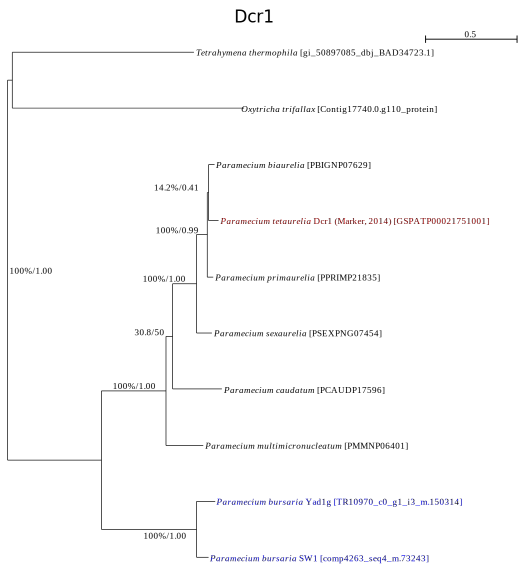
\includegraphics[width=\textwidth]{Dcr1.pdf}
    \caption[RAxMl 1000 bootstraps MrBayes PP]{}
    \label{fig:dcr1}
\end{figure}


\subsubsection{Pds1}

There were no hits for Pds1 in any of the 3 \textit{P. bursaria} datasets 
(both transcriptomes and the genome).  
There were homologues in each of the other \textit{Paramecium} species
i.e. \textit{P. sexaurelia}, \textit{P. biaurelia}, \textit{P. primaurelia},
\textit{P. multimicronucleatum} and \textit{P. caudatum} but not
\textit{T. thermophila} or \textit{O. trifallax}.
\begin{figure}
    \includegraphics[width=\textwidth]{Psd1_tree.pdf}
    \caption[Phylogeny of Pds1 Sequences]{RAxML phylogeny with 1000 non-rapid
        bootstraps annotated with MrBayes (2,000,000 generations) PP. LG This shows that Pds1 homologues
in the \textit{Paramecium} clade largely recapitulates the etablished
\textit{Paramecium} phylogeny.  \textit{P. caudatum}-\textit{P. multimicronucleatum}}
\label{fig:pds1}
\end{figure}

The structure of Pds1 was predicted from the \textit{P. tetaurelia}
sequence via RaptorX (\cref{fig:pds1_struct}).  
Unfortunately, there were no likely predicted functions
from this structure. No structural hits were found aginst known enzyme active sites, ligand-binding
sites or DNA-binding templates in ProcFun.


\begin{figure}
    \includegraphics[width=\textwidth]{psd1_struct.png}
    \caption[Predicted Structure of Pds1]{RaptorX Predicted Structure of \textit{P. tetaurelia}
    Pds1 protein (PTETP600032001). No functional annotations could be made using this structure}
    \label{fig:pds1_struct}
\end{figure}

\subsubsection{Cid}

There was a single Cid homologue present in each transcriptome
and a single gene identifiable in the genome. 
Upon alignment the \textit{P. bursaria} SW-1 copies
proved near identical with clear intronic sequences.

Phylogenetic analysis (\cref{fig:cid_phylo}) demonstrated
the existence of a pre-duplication homologue to the Cid1 and Cid2
paralogues present in the rest of the \textit{Paramecium} clade.

\begin{figure}
    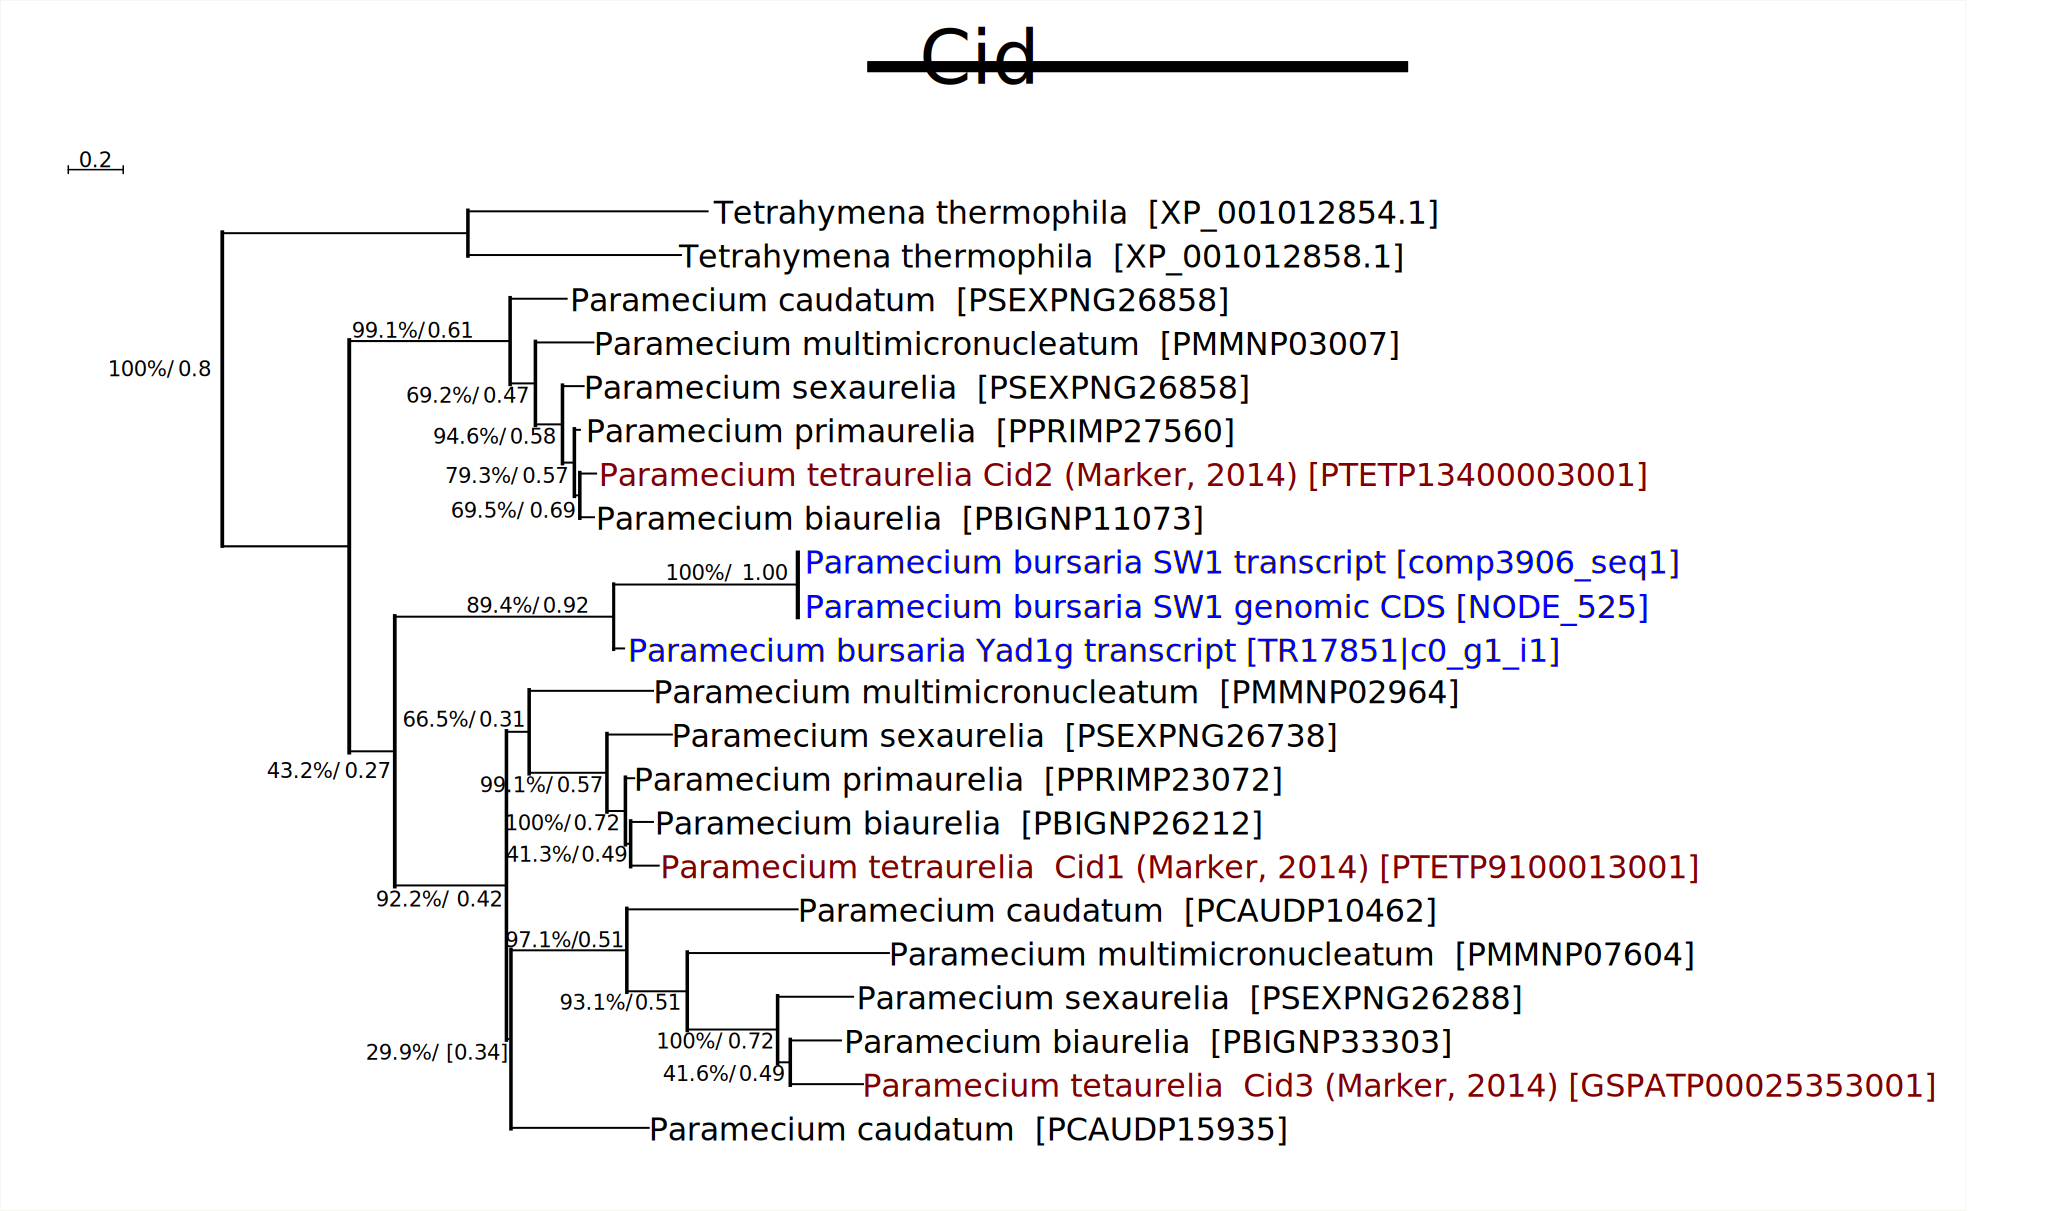
\includegraphics[width=\textwidth]{Cid.pdf}
    \caption[Phylogeny of Cid Sequences]{RAxML phylogeny annotated
    with MrBayes PP showing the existence of a single homologue
of the Cid1 and Cid2 proteins in \textit{P. bursaria}}
    \label{fig:cid_phlyo}
\end{figure}

\subsubsection{Rdr}

\begin{figure}
    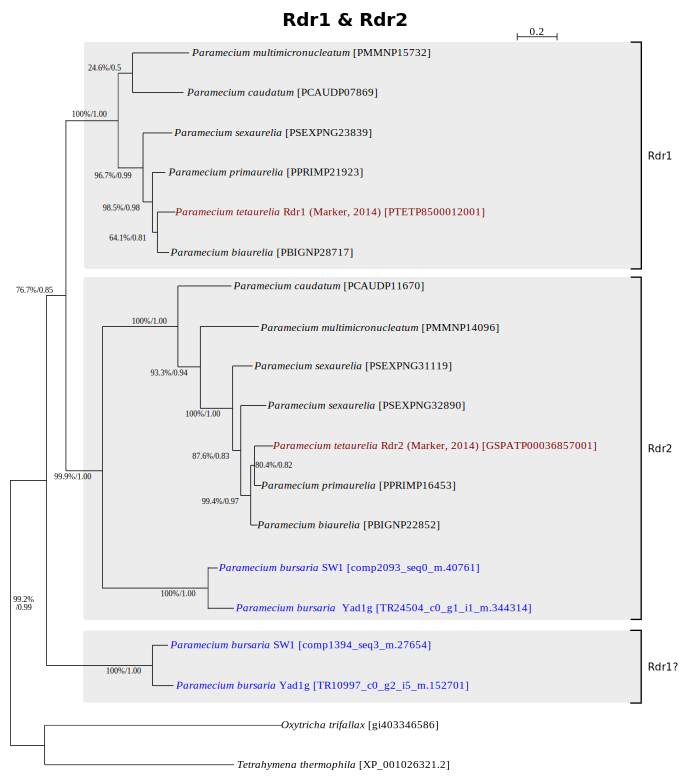
\includegraphics[width=\textwidth]{Rdr1_2.pdf}
    \caption[Phylogeny of Cid Sequences]{RAxML
        phylogeny 
    and Likelihood phylogeny of CID components.}

    \label{fig:rdr_phylo}
\end{figure}


\begin{figure}
    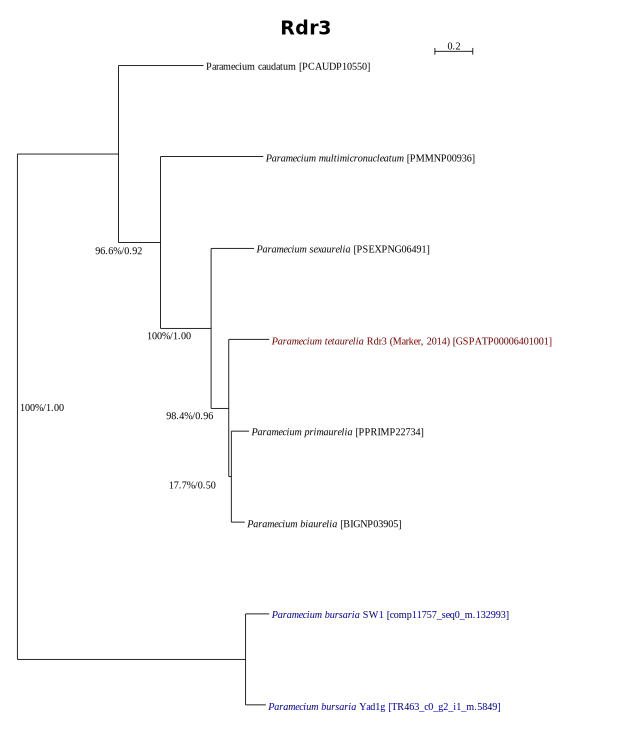
\includegraphics[width=\textwidth]{Rdr3.pdf}
    \caption[Phylogeny of Cid Sequences]{RAxML
        phylogeny 
    and Likelihood phylogeny of CID components}
    \label{fig:rdr_phylo}
\end{figure}



\subsubsection{Piwi}

There were a large number of Piwi detected homologues across
the datasets. Specifically, 16 Piwi in the \textit{P. bursaria} SW-1
transcriptome and 5 in the partial genome, and 17 in the \textit{P. 
bursaria} Yad1g transcriptome.
Due to the large size of this family, large number of paralogues
and relatively short sequences phylogenetic inference
of these sequences proved largely intractable. There are Piwi
homologues present in \textit{P. bursaria} although their exact
relation and function is unknown.


\subsection{RNAi cross-talk}

The total number of unique collisions between the endosymbionts and 
the various classes of subject predicted transcriptomes were plotted
(\cref{fig:unique_collisions}).  This showed that there 
were next to collisions with Archaea and the endosymbionts but were
low levels of collision with Bacteria.  Eukaryotes in general
lead to much higher levels of collision.  Green algae
had the most collisions as might be expected from their close
relationship with the green algal endosymbiont. Interestingly,
the 3 ciliate species had a low number of collisions but there
was moderate to high levels of collision against the two
\textit{P. bursaria} host transcriptomes.

\begin{figure}
    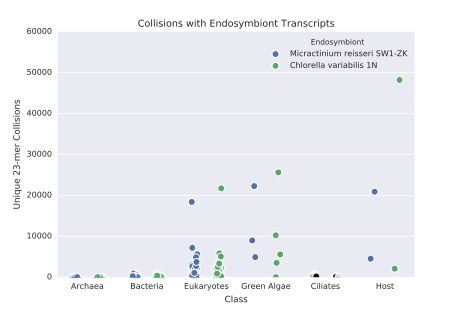
\includegraphics[width=\textwidth]{unique_collisions.pdf}
    \caption[Unique eDicer Collisions by Subject Class]{The number of unique 23-mer
        between transcripts from the \textit{C. variabilis} 1N
    and \textit{M. reisseri} SW1-ZK endosymbionts and different
classes of subject transcripts.  The only sequences with more than 6000
unique collisions were \textit{Coccomyxa variabilis} NC64A and \textit{Chlorella subellipsoidea} C-169
, \textit{Arabidopsis thaliana}, \textit{Chlamydomonas reinhardtii} and transcripts
from the two host bins \textit{P. bursaria} SW1 and \textit{P. bursaria} Yad1g.  
This suggests RNAi-cross talk could be occurring between the host and endosymbiont}
\label{fig:unique_collisions}
\end{figure}

In order to test to what degree the number of collisions was related
to the length of the subject query linear regression was conducted
using all points (\cref{fig:edicer_collisions_by_length}).  This
demonstrates there is at least a partial linear dependence between the 
length of the query and the number of collisions.

\begin{figure}
    \centering
    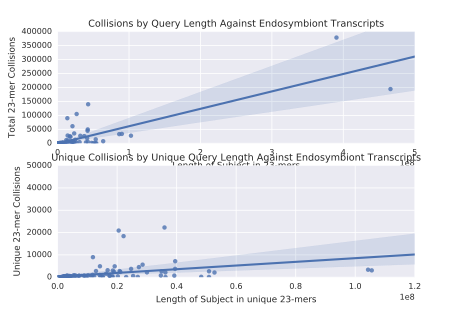
\includegraphics[width=\textwidth]{length_collisions_regs.pdf}
    \caption[Regression of eDicer Collisions by Query Length]{Linear Regressions
    of the relationship between the number of collisions as query length
increases. Features points from collisions with both \textit{C. variabilis} 1N
and \textit{M. reissier} SW1-ZK.  Dark blue cloud indicates \(95\%\) confidence
intervals.  
The top plot shows total collisions against
total length whereas the bottom analysis only looks at unique collisions
against unique length so theoretically ameliorates the effect of repetitative 
transcripts/many isoforms.  Both show a clear linear relationship and thus
indicate the importance of normalising by query length in an analysis of 
collisions.}
    \label{fig:edicer_collisions_by_length}
\end{figure}


Normalising the unique number of collisions by the unique length of
the subject predicted transcriptome led to some interesting results (\cref{fig:edicer_uniq_norm})
Collisions with Eukaryotes largely were reduced to being on-pair
with collisions with Bacteria. 
Despite collisions against the Ciliates relatively disappearing,
there was still considerable levels of collision against
the host transcriptomes and green algae.

\begin{figure}
    \centering
    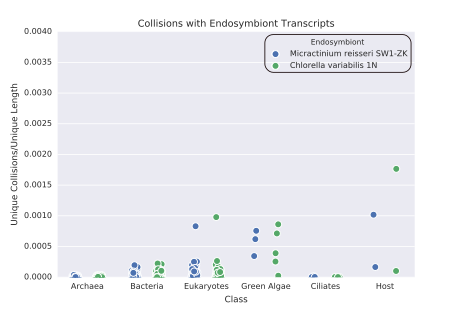
\includegraphics[width=\textwidth]{unique_norm_collisions.pdf}
    \caption[Normalised Unique eDicer Collisions]{The number of collisions
        between transcripts from the \textit{C. variabilis} 1N
    and \textit{M. reisseri} SW1-ZK endosymbionts and different
classes of subject transcripts normalised by the unique length of those
subjects.}
    \label{fig:edicer_unique_norm}
\end{figure}


\section{Discussion}


\subsection{No dsRNA RNAi inducible phenotypes in \textit{P. bursaria} SW1}

Despite numerous attempts all feeding experiments failed to induce
any of the RNAi knockout phenotypes.  RT-PCR tests with the Bug22
and BBS7 constructs demonstrated
that the \textit{E. coli} were expressing the dsRNA.  
This indicates that dsRNA is either incapable of escaping the digestive vacuole
or the host does not have an active pathway for exogenous dsRNA incuded
RNAi.  The the fact that microinjection of dsRNA directly into the MAC
also failed to elicit RNAi phenotypes would support the absence
of an active dsRNA induced RNAi pathway. 

However, the high methodological difficulty involved in identifying and injecting
the MAC without lysing the cell (\cref{fig:microinjection_nucleus}) 
means microinjection may have only failed to induce RNAi due to failure
to correctly microinject \textit{P. bursaria}.   \textit{P. bursaria}
was particularly prone to lysis relative to \textit{P. tetaurelia} and
there were greater issues with trichocysts blocking the microinjector. 
Attempts made to inject GFP into the MAC to observe whether microinjection
was taking place also failed supporting a technical failure of this
approach rather than necessarily a biological reason.

\begin{figure}
    \includegraphics[width=\textwidth]{microinjection_hard.pdf}
    \caption[DAPI Stained \textit{P. bursaria} MAC]{DAPI stained \textit{P. bursaria}
        MAC to demonstrating how difficult it is to accurately identify the limits
    of the MAC for microinjection}
    \label{fig:microinjection_nucleus}
\end{figure}

Unfortunately, microinjection is also a necessary stage in the transgene
induced RNAi methodology.  Therefore, even if this alternative pathway
is present and active it may still not be possible to reliably 
induce RNAi in \textit{P. bursaria}.


\subsection{Missing components of RNAi pathway in \textit{P. bursaria}}

There are several components missing that are required for the function
of the exogenous dsRNA RNAi pathway in \textit{P. tetaurelia}.

Pds1 is totally absent outside of the \textit{Paramecium} clade post the divergence
of \textit{P. bursaria} and \textit{P. caudatum}.  A phylogenetic
analysis of Pds1 sequences (\cref{fig:pds1}) recapitulated the established 
\textit{Paramecium} taxonomy (\cref{fig:paramecium_genomes}).
This suggests that Pds1 was either acquired after the divergence of \textit{P. bursaria}
and \textit{P. caudatum} or was lost in \textit{P. bursaria}.
The pattern of paralogues would more likely support the former scenario.
The lack of paralogues (with the exception of a terminally duplicated \textit{P. multimicronucleatum}
copy) in the \textit{P. aurelia} complex species is interesting.  As the presence
of Pds1 in \textit{P. caudatum} indicates that this should have undergone
duplication during the 2 subsequent WGD events.  Potentially, this represents
serial losses in these species.

It is possible that Pds1 is present and just hasn't been recovered 
in the partial transcriptomes because it is not being transcribed (or is 
transcribed at a very low level) during endosymbiosis.  It is also
possible it is missing in the partial genome due to the incompleteness
of this data.  However, the combination of being missing in all 3 datasets
as well as any non-\textit{Paramecium} ciliates indicates that
it is likely not present in \textit{P. bursaria}.

However, a single copy of the Cid protein was present in \textit{P. bursaria}.
The fact that there are two copies in \textit{P. caudatum} (which 
shares the ancient WGD with \textit{P. bursaria}) indicates the possiblity
of the loss of Cid2 in \textit{P. bursaria}.
The putative Cid1 in \textit{P. bursaria} may be functional in the common
RNAi pathway.

The unresolved Piwis 


Ultimately, based on the missing components of the RNAi pathways
identified in \textit{P. tetaurelia} this indicates that the exogenous dsRNA
pathway is likely to not be active.  Unless Cid2 is functional in the shared
RNAi pathway then it is possible that the both pathways identified in \textit{P. tetaurelia}
are not active in \textit{P. bursaria}.  

\subsection{Endosymbiont ``collision'' hypothesis}

Exogenous RNAi response is not essential for viability in \textit{P. tetaurelia}
\citep{Marker2014}.

However, the high degree of conservation even in \textit{P. bursaria}
suggests they play an important role. 

No \textit{Paramecium} viruses have been identified yet. 

Prseumably they exist, however it is possible that the endosymbiont plays a role.


\textit{C. elegans} has a dsRNA transporter (\textit{SID-2}) \citep{Nuez2012}


microinjection of fluore

often bursts after 1 injection, trichocysts block needle





Hypothetically, one explanation for the deactivation/loss
of RNAi in \textit{P. bursaria} CCAP 1660/12.


A regression analysis using a measure of phylogenetic distance would be interesting.
For example k-mer collisions by 100


Only finds exact matches though.


Finally, while this may not have thoroughly resolved the question of matches
eDicer may form a useful tool in the rapid screening of off-target effects
in the RNAi analyses in different organisms.   It is considerably
more efficient than exact matches 
than cut and alignment based methods. 





\section{Conclusions}

RNAi induced phenotypes could not be created in \textit{P. bursaria} CCAP1660/12
by either feeding experiments or direct transgene microinjection. 

Therefore, assembled transcriptomic and genomic data from \textit{P. bursaria}
CCAP 1660/12 and YADG1N were analysed for factors identified as essential in the function
of these pathways in \textit{P. tetaurelia} \citep{Marker2014}. 

\begin{figure}
    \includegraphics[width=\textwidth]{RNAi_factors_summary_figure.pdf}
    \caption[Summary of RNAi Factors Presence]{Summary of the discovery
    of RNAi figures in \textit{P. bursaria}}
    \label{fig:rnai_summary}
\end{figure}

Two proteins essential for the function of the exogenous dsRNA induced
RNAi pathway in \textit{P. tetaurelia}, Pds1 and Rdr1, were not found in the partial genome and transcriptome 
of \textit{P. bursaria} CCAP 1660/12 or the transcriptome of \textit{P. bursaria} YADG1N.
This suggests that this pathway may not be active/present in \textit{P. bursaria}.
Either, 


However, assuming the likely pre-duplication orthologue of Cid2 and the necessary 
unresolved Ptiwi's are functional
in the transgene dsRNA pathway of \textit{P. bursaria}
then this pathway is theoretically active.  Unfortunately, methodological
difficulties in microinjection have thus far failed to generate RNAi-induced
phenotypes.
